\chapter{Test and beam time analysis} \label{analysis}

\begin{outline}[enumerate]
\1 development of the analysis program (description of the Levenberg-Marquardt-Algorithmus.
\1 testing the analysis program with montecarlo data.
\1 Test of the detectors in the Lab.
\1 Beam line description.
\1 Data Analysis
	\2 Rates on $Pb^{208}$.
	\2 Stabilization Monitors.
	\2 $C^{12}$ Asymmetry.
\end{outline}

\section{Model for fitting the data}
Here I have to explain the model used for describing the data, so the problem of the false asymmetry induced by variations in beam position, angle, current and energy. Here is a good point to explain the De Brujin sequence for the polarity patterns

\section{Data tree}
Explain how we compute all the values for the data tree, the position of the beam on the target, the angle, the correlated-difference values...

\section{Detectors test}
Explain the test of the two detectors in the lab, how we select the threshold, the correlation of the pmts and coincidence to select the threshold

\section{Analysis}

\subsection{Alignment of the scattering plane}

\subsection{Calibration of the VFCs monitors}

\subsection{Calibration of the PIMO, Current and ENMO monitors}

For the current monitors I13 and I21, we perform the calibration changing the current of the beam and observing the output values of the monitors (Voltage values). The we perform a fit (for the beam current, we used the nominal values that we communicate to MAMI, has the values for the x-axis).

\begin{figure}[hbtp]
\centering
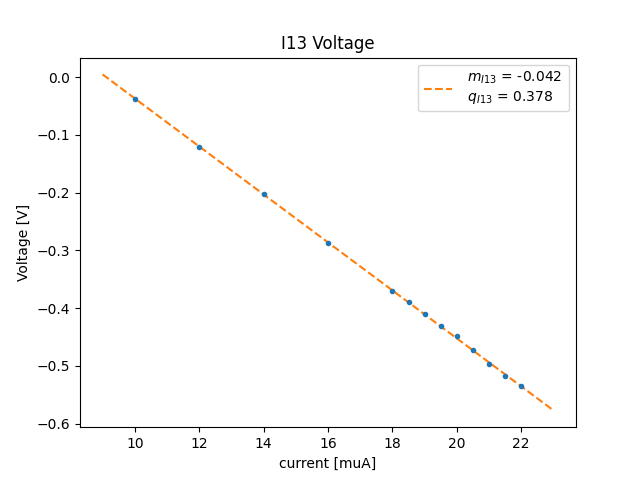
\includegraphics[width = 0.45\textwidth]{Analysis/I13_Calibration.png}
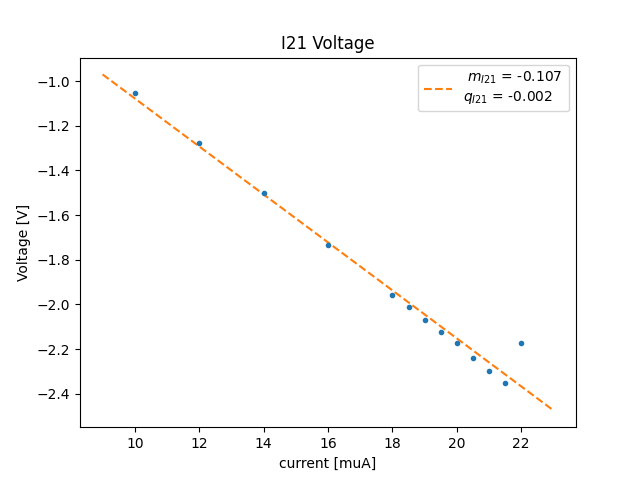
\includegraphics[width = 0.45\textwidth]{Analysis/I21_Calibration.png} 
\caption{•}
\end{figure}

For the two monitors we are able to compute the offset and scale factor:

\begin{equation}
\begin{split}
I^{volt}_{13} = m_{13} \cdot I^{Nom}_{13} + q_{13}\\
c_{13} = \frac{1}{m} \qquad offset = -\frac{q_{13}}{m}
\end{split}
\end{equation}

The same formula for current monitor I21.

The Enmo calibration is performed in a different from the other monitors. The polarity signal is sent to MAMI, and they produce a signal for the ENMO that somehow (need to investigate exactly how they do that) shows a difference between the first two subevents and the last two. This difference is equal (nominal) to $\SI{22.6}{\kilo \electronvolt}$. The idea now is to produce an histogram for the quantity $\delta E$ (with $E_{18}$ being the energy monitor):

\begin{equation*}
\delta E = \frac{E_{18}[2] + E_{18}[3]}{2} - \frac{E_{18}[0] + E_{18}[1]}{2} 
\end{equation*}

3 runs of data where taken with different Beam current. Taking the mean it is possible to exstimate the scaling factor for the ENMO monitors, obtaining the physical quantity in this way.

\begin{equation*}
c_{E18} = \frac{\SI{22.6}{\kilo \electronvolt}}{\overline{\delta E}}
\end{equation*}

\begin{figure}[hbtp]
\centering
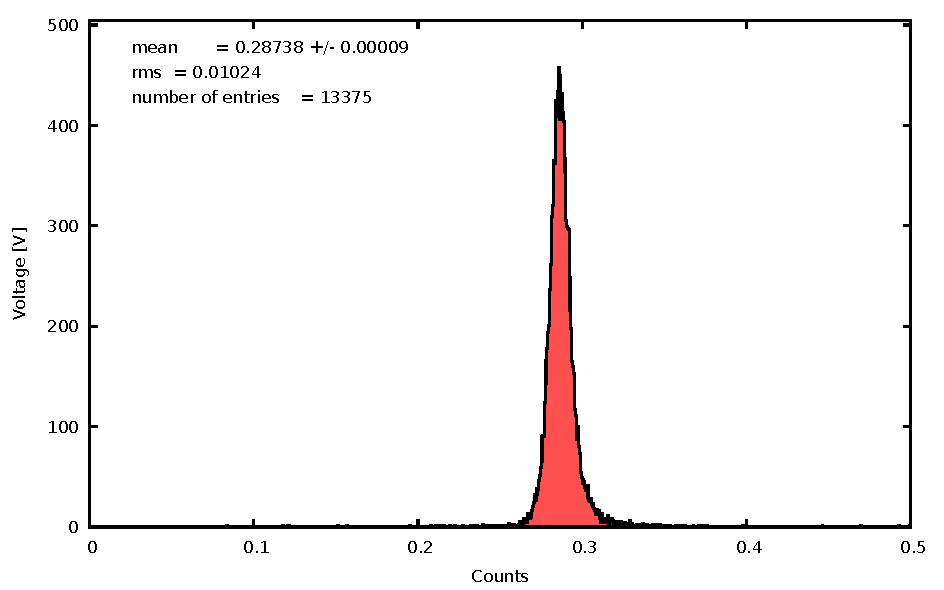
\includegraphics[width = 0.5\textwidth]{Analysis/Enmo_Calibration.pdf}
\caption{$\delta E$ for 20 $\SI{20}{\micro \ampere}$}
\end{figure}

Taking the average over $E_{18}$ voltage values, and using the formula above, we obtain the coefficient $c_{E18}$.
Then, the next step it's to study the dependence of the response of $E_{18}$ on the current.
The calibration was performed taking three acquisitions with different current for the beam current : $\SI{20}{\micro \ampere}$, $\SI{15}{\micro \ampere}$ and a run without beam. 

\begin{figure}[hbtp]
\centering
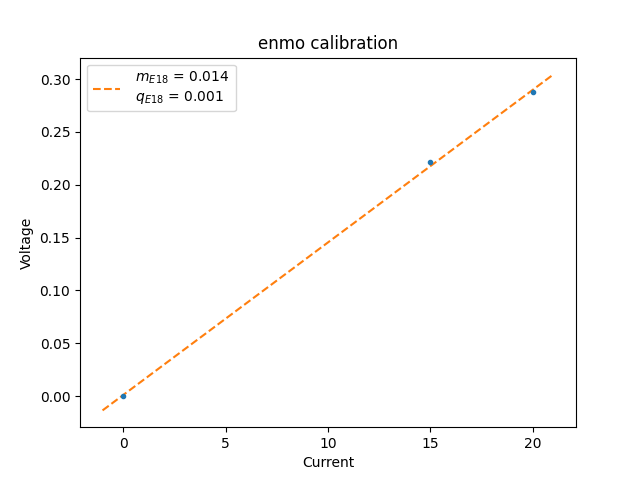
\includegraphics[width = 0.5\textwidth]{Analysis/E18_Calibration.png}
\caption{Calibration of ENMO monitor}
\end{figure}




\subsection{Calibration of the pmts}

\subsection{Rates on lead}

\section{ $^{12}C$ asymmetry}

\subsection{least square fit}

\subsection{False asymmetries}

\subsection{??Boostrap??}

\subsection{??interval estimation??}




